%%
%% LogsheetXtractor — SoftwareX manuscript
%% Adapted from softwarex-osp-template.tex and content from paper.md
%%

\documentclass[preprint,12pt,a4paper]{elsarticle}

\usepackage{amssymb}
\usepackage{hyperref}
\usepackage{booktabs}
\usepackage{listings}
\lstset{
  basicstyle=\ttfamily\small,
  breaklines=true,
  columns=fullflexible,
  frame=single,
  language=bash
}
\setlength{\parindent}{0pt}

\journal{SoftwareX}

\begin{document}
\renewcommand{\labelenumii}{\arabic{enumi}.\arabic{enumii}}

\begin{frontmatter}

\title{LogsheetXtractor: A web application for digitizing handwritten field logsheets}

%% Authors and affiliations (from paper.md)
\author[embl]{Matej Troj\'{a}k\corref{cor1}}
%% TODO: corresponding-author email
\ead{matej.trojak@embl.de}
\cortext[cor1]{Corresponding author}

\author[masaryk]{Jan Glos}

\author[ebi]{St\'{e}phane Pesant}

\author[embl]{Kerstin Leberecht}

\author[embl]{Michael Kuhn}

\author[embl]{Peer Bork}

\address[embl]{EMBL, Heidelberg, Germany}
\address[ebi]{EMBL-EBI, Hinxton, UK}
\address[masaryk]{Masaryk University, Czech Republic}
%% TODO: confirm affiliation wording / postal addresses if required by SoftwareX

\begin{abstract}
Field research often relies on paper logsheets that are durable in harsh environments but cumbersome to digitize afterward.
The open-source tool formHTR automates extraction of handwritten values from scanned forms using template-defined regions of interest (ROIs) and external OCR services, but its command-line workflow is difficult for non-technical domain experts.
LogsheetXtractor is a full-stack web application that wraps formHTR in a browser-based workflow for template management, logsheet upload, alignment, OCR processing, proofreading, and export to spreadsheet formats.
The software targets research teams---initially motivated by coastal biodiversity fieldwork on the TRaversing European Coastlines (TREC) expedition---who need structured digital data without maintaining local Python environments.
\end{abstract}

\begin{keyword}
OCR \sep HTR \sep document digitization \sep web application \sep biodiversity \sep field research
\end{keyword}

\end{frontmatter}

%% =====================================================================
%% Required metadata
%% =====================================================================

\section*{Required Metadata}
\label{sec:metadata}

\section*{Current code version}
\label{sec:code-version}

Ancillary data table required for subversion of the codebase.

\begin{table}[!h]
\begin{tabular}{|l|p{6.5cm}|p{6.5cm}|}
\hline
\textbf{Nr.} & \textbf{Code metadata description} & \textbf{Please fill in this column} \\
\hline
C1 & Current code version & TODO: release/tag (e.g.\ v1.0.0) \\
\hline
C2 & Permanent GitHub link to code/repository used for this code version & \url{https://github.com/grp-bork/LogsheetXtractor} \\
%% TODO: confirm canonical public GitHub URL before submission (SoftwareX requires GitHub)
\hline
C3 & Legal Code License & MIT \\
\hline
C4 & Code versioning system used & git \\
\hline
C5 & Software code languages, tools, and services used & C\# / ASP.NET Core, TypeScript / React, Python (formHTR), Docker Compose; OCR via Amazon Textract, Google Cloud Vision, or Azure AI Vision \\
\hline
C6 & Compilation requirements, operating environments \& dependencies & Docker Desktop (recommended); or .NET SDK, Node.js, and Python with formHTR for non-container development. See repository README. \\
\hline
C7 & If available Link to developer documentation/manual & \url{https://github.com/grp-bork/LogsheetXtractor} (README and component guides) \\
%% TODO: add dedicated docs URL if published separately
\hline
C8 & Support email for questions & TODO: support / contact email \\
\hline
\end{tabular}
\caption{Code metadata (mandatory)}
\label{tab:code-metadata}
\end{table}

%% =====================================================================
%% Main text (SoftwareX required sections)
%% =====================================================================

%% ---------------------------------------------------------------------
\section{Motivation and significance}
\label{sec:motivation}
%% ---------------------------------------------------------------------

Field research often relies on paper logsheets that are durable in harsh environments but cumbersome to digitize afterward.
Paper-based data collection remains practical where power, connectivity, or training constraints rule out digital devices in the field~\cite{walther11,VANTAMELEN2004123,BREWER2016131}.
Once scans are available, however, manual transcription and error-prone spreadsheet proofreading become bottlenecks.

The open-source Python tool formHTR~\cite{formHTR_repo} automates extraction of handwritten values from scanned forms using template-defined regions of interest (ROIs) and external optical character recognition (OCR) services~\cite{ocr156468} such as Amazon Textract, Google Cloud Vision, or Azure AI Document Intelligence~\cite{amazon_textract,google_vision_api,azure_form_recognizer}.
Its command-line workflow is difficult for non-technical domain experts: users must install Python, manage virtual environments, distribute API credential files, and verify flat spreadsheet output against original scans without built-in spatial context.

LogsheetXtractor is a full-stack web application that wraps formHTR in a browser-based workflow for template management, logsheet upload, alignment, OCR processing, proofreading, and export to spreadsheet formats.
The software targets research teams---initially motivated by coastal biodiversity fieldwork on the TRaversing European Coastlines (TREC) expedition~\cite{embl_trec}---who need to move from paper capture to structured digital data without maintaining local Python environments or juggling separate tools for verification.

\paragraph{Contribution to scientific discovery.}
By lowering the barrier to digitizing handwritten field forms, LogsheetXtractor helps research programmes convert paper archives into structured, validated datasets suitable for curation and reuse (e.g.\ metaTREC coordinate validation workflows~\cite{metaTREC_curation}).
%% TODO: cite a research paper that used the software, if/when available.

\paragraph{Experimental setting / how users use the software.}
Administrators configure OCR credentials on a centralized deployment.
Researchers then: (i)~upload or select a PDF template and define typed ROIs; (ii)~upload scanned logsheets; (iii)~align each scan to the template (automatic and/or manual); (iv)~run OCR; (v)~proofread extracted values side-by-side with the scan; and (vi)~export corrected data to spreadsheet formats. The command line Python tool can be used by an advanced user to perform these actions as well.

\paragraph{Related work.}
Several ecosystems address parts of the handwritten-form digitization problem, but none fully match the combined requirements of template versioning, multi-provider OCR orchestration, and integrated proofreading for irregular field scans.

\textbf{formHTR}~\cite{formHTR_repo} is the direct predecessor and extraction engine.
It is mature for batch processing and offers desktop GUIs for ROI selection, yet configuration remains file-based, processing is script-driven, and verification happens outside the tool in Excel.
Contributing only to formHTR would not deliver a shared web deployment, real-time processing notifications, or the linked proofreading workspace described below.

\textbf{Open-source OCR engines} such as Tesseract~\cite{tesseract_ocr}, EasyOCR~\cite{easyocr}, OCR4all~\cite{app9224853}, and PaddleOCR~\cite{cui2025paddleocr30technicalreport} provide pretrained models (and, in some cases, custom training), with trade-offs in accuracy, speed, and deployment complexity.
\textbf{Cloud document-AI services} including Google Cloud Vision~\cite{google_vision_api}, Azure AI Document Intelligence~\cite{azure_form_recognizer}, and Amazon Textract~\cite{amazon_textract} are highly optimised for structured documents and can return higher-level outputs (e.g.\ key--value pairs), but they do not manage template libraries, logsheet lifecycle states, ROI semantics (numeric fields, checkboxes, barcodes), or domain-specific validation such as geographic coordinate bounds~\cite{metaTREC_curation}.

\textbf{Multi-engine wrappers} such as OCRmyPDF~\cite{ocrmypdf}, OcrPy~\cite{ocrpy}, and Handprint~\cite{handprint} abstract over several backends or compare cloud handwriting services, yet they are not oriented toward versioned form templates, ROI-typed field extraction, or an end-to-end web proofreading workspace for expedition logsheets.
Handprint in particular is no longer maintained.

\textbf{Electronic data capture (EDC) and mobile form apps} replace paper at collection time~\cite{VANTAMELEN2004123,BREWER2016131}.
They are ill-suited when waterproof paper, offline field conditions, or expedition logistics require physical sheets first.

\textbf{Spreadsheet-centric workflows} remain the de facto verification path for many labs but amplify context switching between PDF viewers and tables, which user testing linked to missed OCR corrections (see Section~\ref{sec:impact}).

LogsheetXtractor was built as a web orchestration layer on top of formHTR because the research community already depended on the Python extraction pipeline, while the missing capability was an accessible, deployable interface---not a second OCR implementation.
Upstream changes were contributed to formHTR (e.g., headless ROI detection and web-oriented CLI options) so the CLI and web tool stay aligned~\cite{formHTR_pr81}.

%% ---------------------------------------------------------------------
\section{Software description}
\label{sec:software-description}
%% ---------------------------------------------------------------------

LogsheetXtractor provides a centralized deployment where administrators configure OCR credentials on the server, while researchers interact through a visual interface.
The application preserves formHTR's extraction logic by invoking the existing scripts in isolated processes rather than reimplementing OCR pipelines, so improvements to formHTR continue to benefit both interfaces~\cite{formHTR_pr81}.

\subsection{Underlying formHTR pipeline}
\label{sec:formhtr}

formHTR~\cite{formHTR_repo} is the Python extraction engine that LogsheetXtractor orchestrates.
While recognition itself uses pretrained cloud OCR models, a key design choice is to exploit prior knowledge of each form: users annotate regions of interest (ROIs) on a blank template, assigning locations, variable names, and content types.
Combining that template specification with outputs from multiple OCR providers substantially improves extraction quality relative to unconstrained full-page recognition.

The pipeline has two main stages (Figure~\ref{fig:formhtr-overview}).
In the \emph{specification} step, ROIs are selected on the template and annotated with names and types; the result is a configuration file of positions, names, and types.
In the \emph{processing} step, each scanned logsheet is aligned to its template so that ROI coordinates match the handwriting on the scan.
Alignment can be automatic; when fiducial markers are absent or scan quality is poor, manual alignment is also supported.
The aligned page is then sent to one or more cloud OCR APIs---Google Cloud Vision, Azure AI Document Intelligence, and Amazon Textract~\cite{google_vision_api,azure_form_recognizer,amazon_textract}---each of which returns detected words with bounding boxes.

\begin{figure}[!ht]
\centering
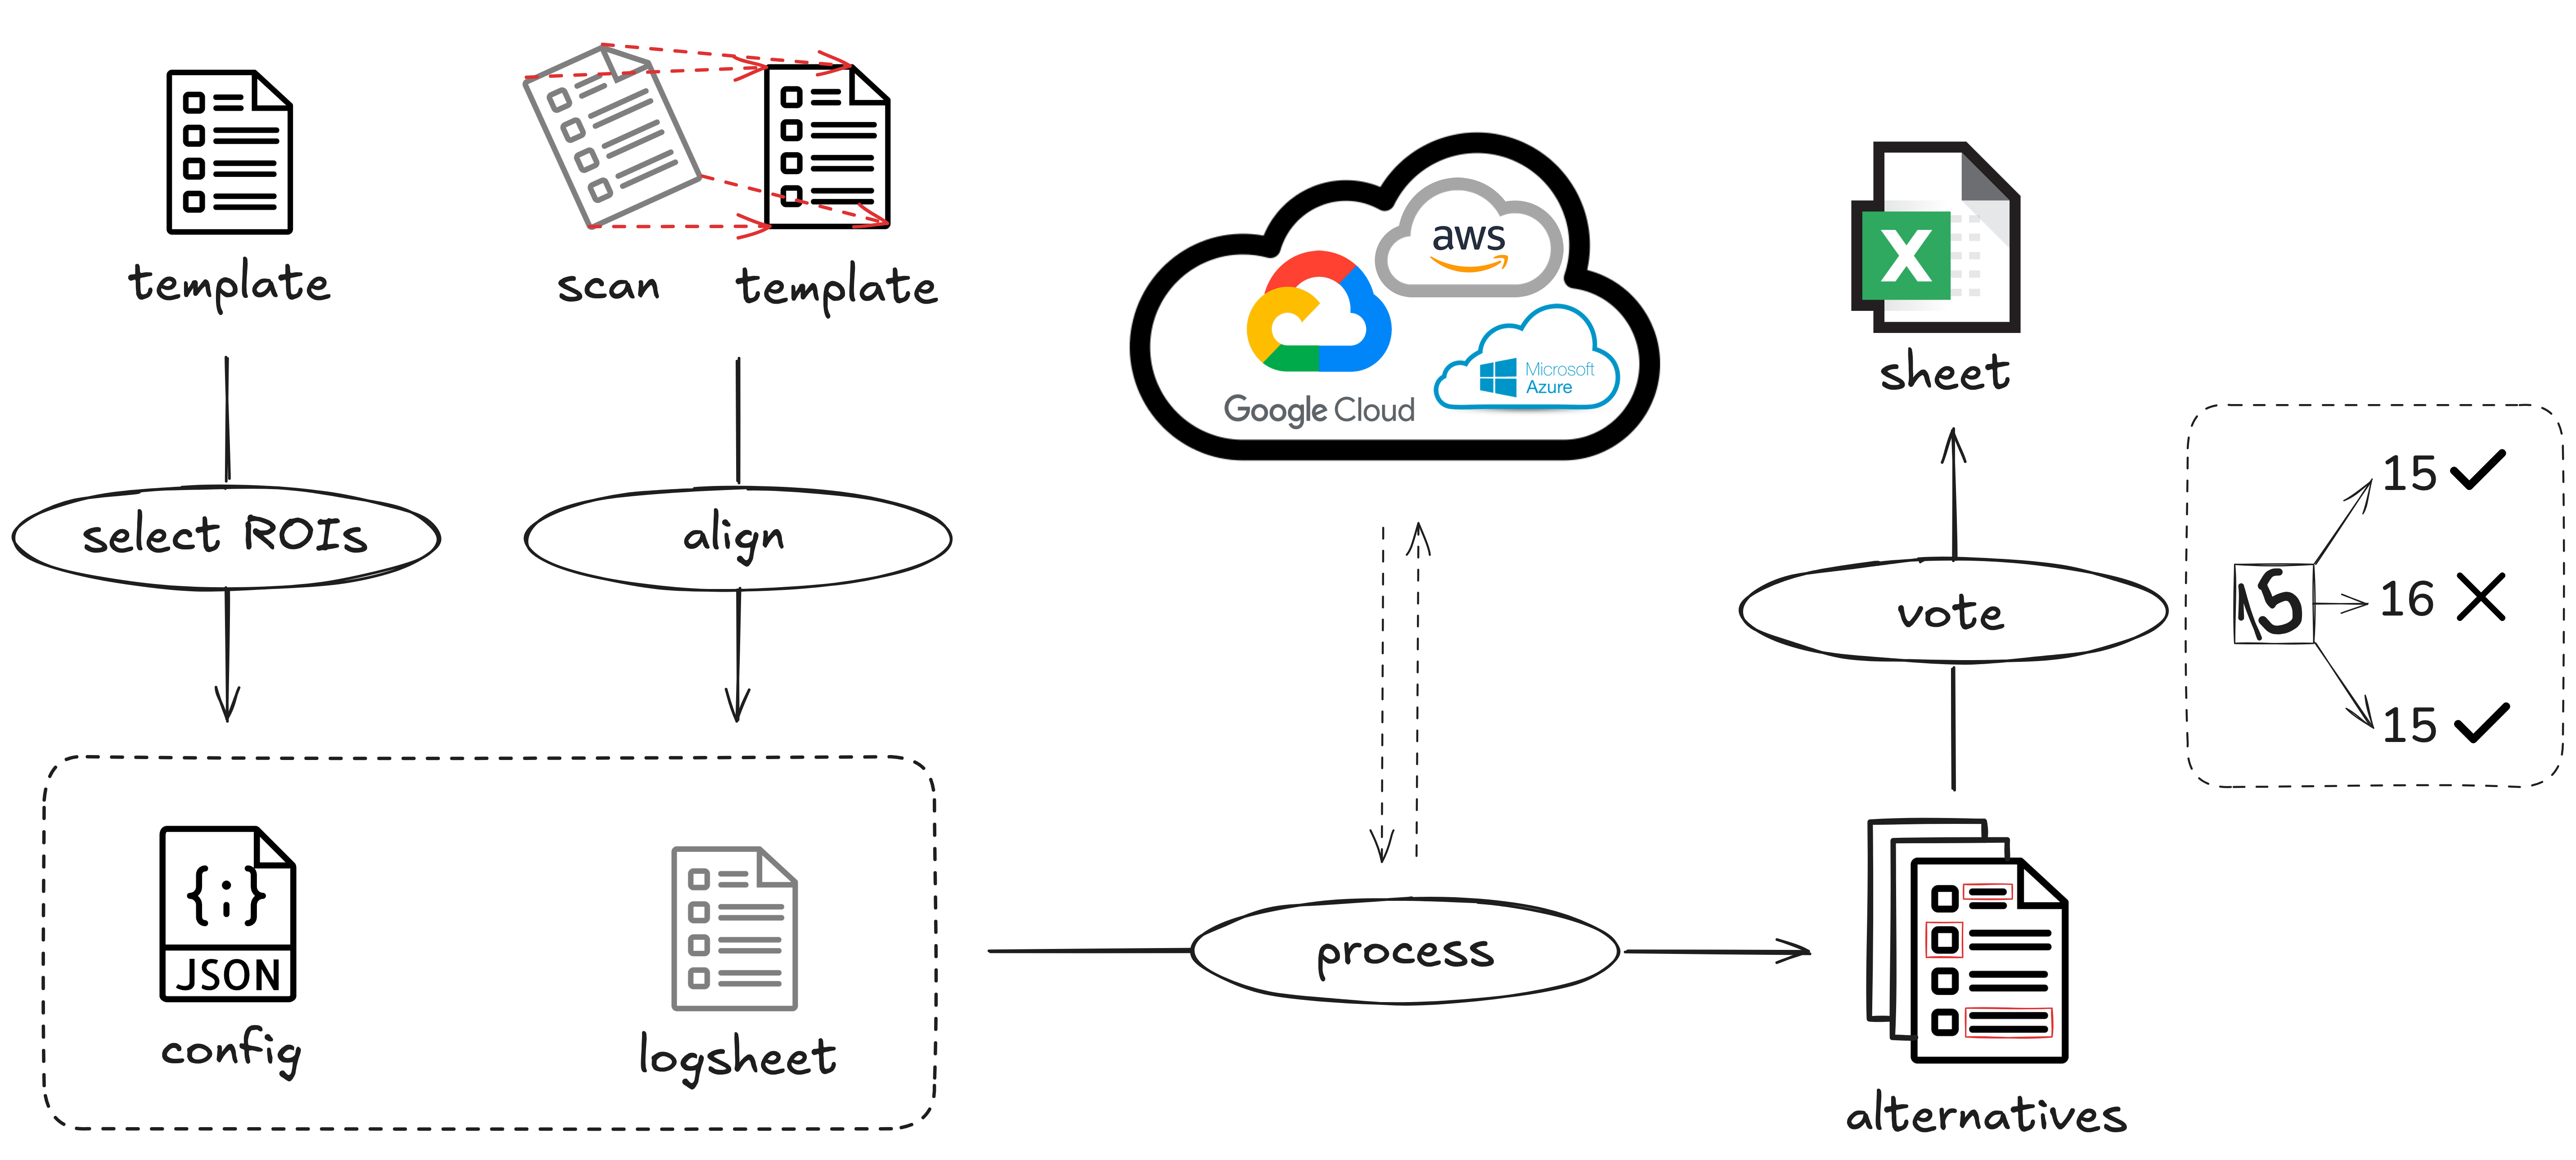
\includegraphics[width=0.95\textwidth]{figures/scheme.png}
\caption{Schematic overview of the formHTR annotation and processing workflow: ROI configuration on a template, alignment of a scan, multi-provider OCR, consensus voting, and spreadsheet export.}
\label{fig:formhtr-overview}
\end{figure}

Detected words are assigned to ROIs by a \emph{binning} step.
Several geometric cases arise in practice: a word spanning multiple ROIs, multiple words overlapping a single ROI, or a sentence split into several tokens (Figure~\ref{fig:binning}).
Overlaps are indexed with an R-tree~\cite{rtree} so intersections between service outputs and template ROIs can be queried efficiently.
Preprinted template text (\emph{residuals}) that can drift into ROI boxes under imperfect alignment is declared during specification and excluded from the extracted values.

\begin{figure}[!ht]
\centering
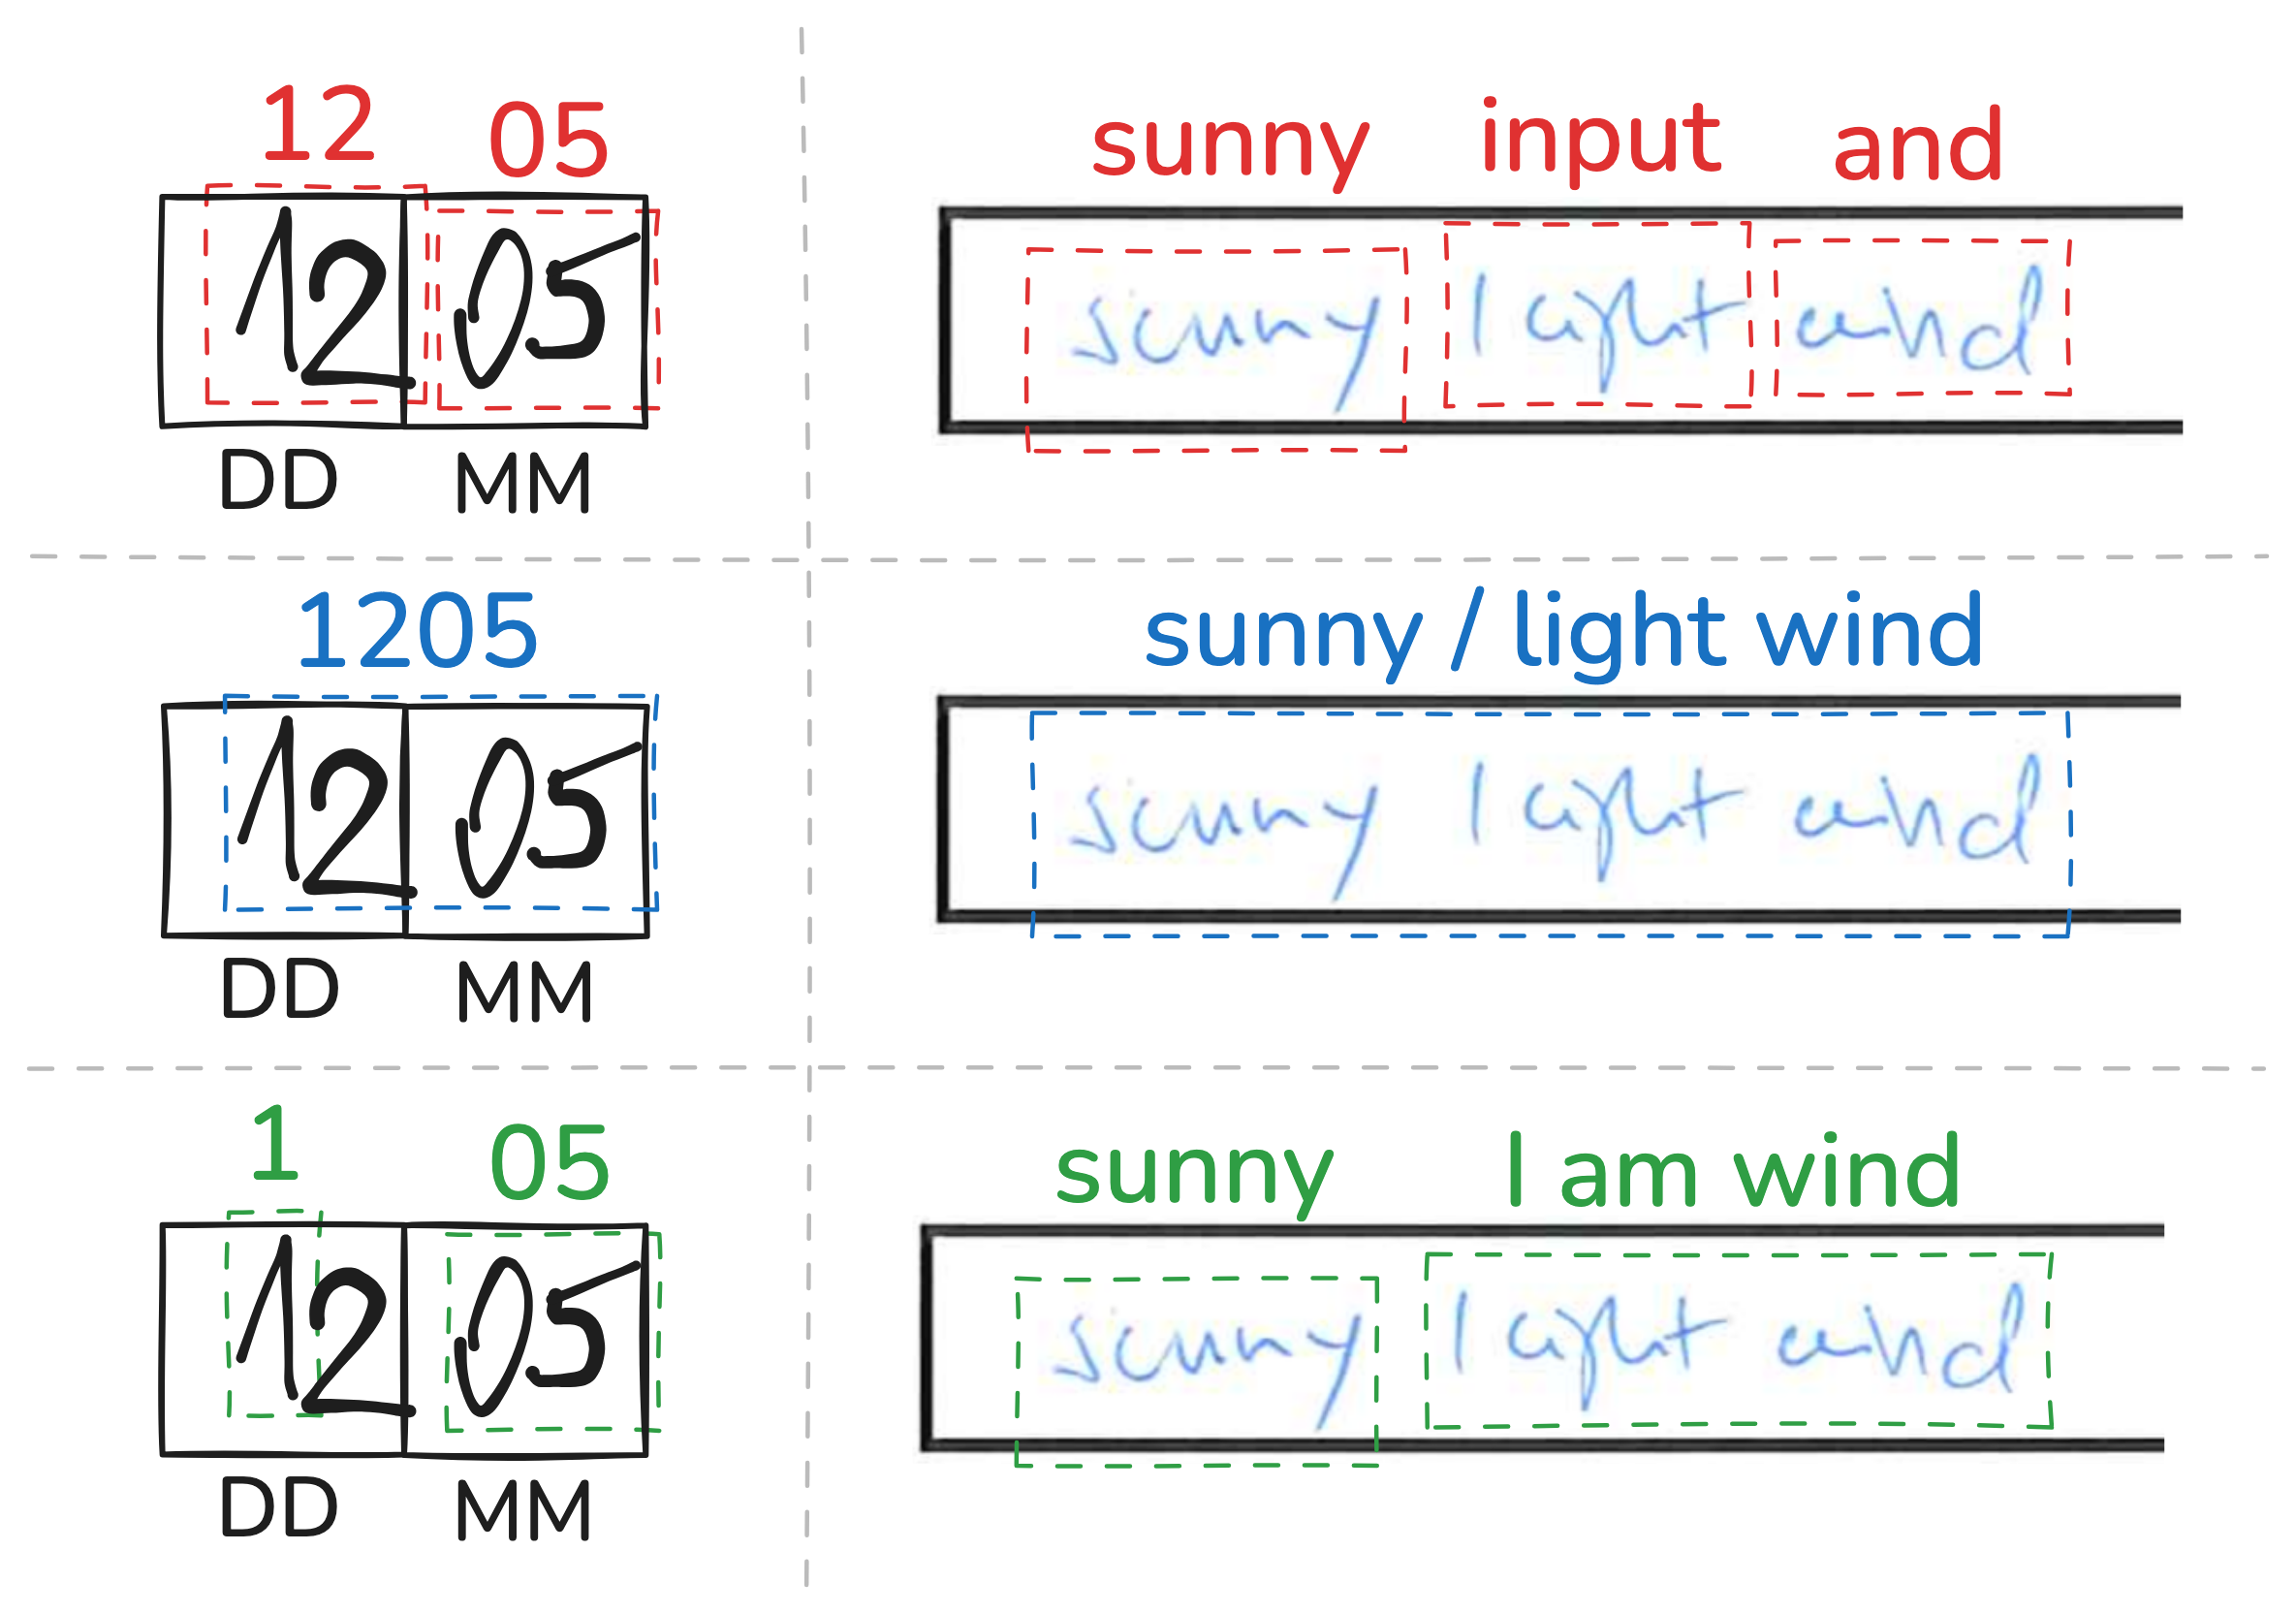
\includegraphics[width=0.95\textwidth]{figures/binning.png}
\caption{Examples of text-to-ROI assignment across OCR services (rows, distinguished by colour).
Left: neighbouring date fields where detections may merge across ROI boundaries or clip digits.
Right: free-text fields where word splitting and recognition differ across services.}
\label{fig:binning}
\end{figure}

When multiple services are enabled, a voting step selects the most likely value per ROI (majority vote with three providers; a random choice if there is no consensus).
Known ROI types can further bias the vote---for example, preferring numerical readings when a numeric field is expected.
With fewer than three services the pipeline still runs, but without full consensus.
The CLI output is an Excel workbook with a \texttt{Metadata} sheet (variable name, voted value, and a cropped ROI thumbnail for proofreading) and an \texttt{Extra} sheet of content that fell outside declared ROIs and residuals---typically margin notes that would otherwise be lost.

\subsection{Software architecture}
\label{sec:architecture}

LogsheetXtractor is a client--server application: a React frontend and an ASP.NET Core backend, packaged with Docker Compose for reproducible deployment.
The design prioritizes process isolation between the web server and formHTR: OCR and image processing run in separate Python subprocesses so failures or heavy workloads cannot take down the API, and dependency conflicts between .NET and Python stacks are avoided.

On the backend, clean-architecture layers (domain, application, infrastructure, API) organize features such as templates, logsheets, ROIs, and extracted values.
CQRS-style commands and queries separate reads from writes; a Wolverine message bus dispatches handlers and domain events (for example, auto-aligning a logsheet after upload) without bloating HTTP endpoints.
Long-running OCR jobs update persisted logsheet state and notify the UI through WebSockets, avoiding fragile client polling.
Predictable business failures use a Result pattern instead of exceptions for control flow.
A transactional outbox ensures database updates and queued processing commands commit atomically.

Integration with formHTR uses a thin script runner and a higher-level adapter that prepares paths, credentials, and headless flags before invoking the Python CLI.
Figure~\ref{fig:architecture} shows the major components.

\begin{figure}[!ht]
\centering
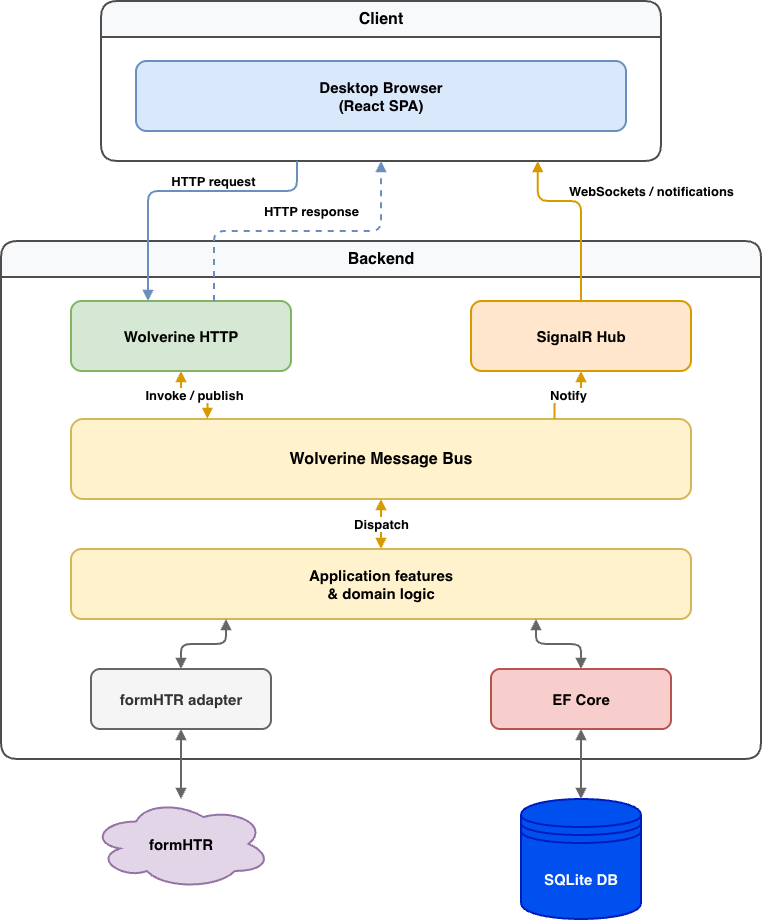
\includegraphics[width=0.95\textwidth]{figures/architecture.png}
\caption{System architecture overview. The browser talks to the ASP.NET API, which persists domain data and delegates OCR alignment and extraction to formHTR while external cloud OCR providers perform recognition.}
\label{fig:architecture}
\end{figure}

The frontend uses TanStack Query for server state, Zod for runtime validation of API payloads, and React context for the template editor.
Automated tests span xUnit unit and integration suites, Vitest and Playwright on the frontend, and API end-to-end tests with a fake script engine so CI does not require live OCR credentials.
GitHub Actions runs these checks on each change.

\subsection{Software functionalities}
\label{sec:functionalities}

Major functionalities include:

\begin{itemize}
  \item \textbf{Template management:} draw, name, and type ROIs on a PDF template; undo/redo history, keyboard shortcuts, and staged saves so frequent ROI edits are not sent on every mouse move.
  \item \textbf{Logsheet lifecycle:} upload scans, track processing state, and persist extracted values.
  \item \textbf{Alignment:} automatic alignment via formHTR, plus manual alignment that overlays a semi-transparent template on the scan; users drag corners until ROIs line up with handwriting, with optional preview of misalignment.
  \item \textbf{OCR orchestration:} run extraction through configured cloud OCR providers without distributing credentials to end-user machines.
  \item \textbf{Proofreading:} split view with logsheet preview and ROI highlights on one side, and a virtualized list of extracted values (cropped ROI thumbnails and editable fields) on the other; selecting an ROI in either pane scrolls and highlights the counterpart.
  \item \textbf{Validation:} optional conditions (type checks, numeric ranges, logical combinations) flag suspicious values before export.
  \item \textbf{Export:} corrected values to spreadsheet formats.
\end{itemize}

\subsection{Sample code snippets analysis}
\label{sec:snippets}

LogsheetXtractor ultimately invokes the same formHTR CLI that domain experts previously ran by hand.
A minimal command-line workflow---ROI selection, annotation, and logsheet processing---is:

\begin{lstlisting}
# 1) Create ROI config for a template
formhtr select-rois --pdf-file template.pdf \
  --output-file config.json

# 2) Annotate ROI types and variable names
formhtr annotate-rois --pdf-file template.pdf \
  --config-file config.json \
  --output-file config_annotated.json

# 3) Process a scanned logsheet
formhtr process-logsheet \
  --pdf-logsheet scan.pdf \
  --pdf-template template.pdf \
  --config-file config_annotated.json \
  --output-file output.xlsx \
  --google google_credentials.json \
  --amazon amazon_credentials.json \
  --azure azure_credentials.json
\end{lstlisting}

In the web application these steps are driven from the UI: the React editor writes and versions the ROI configuration, credentials remain on the server, and the ASP.NET adapter prepares paths and headless flags before spawning the equivalent \texttt{process-logsheet} (and related) invocations in an isolated Python process.
%% TODO (optional): add a short C\# / TypeScript snippet of the adapter if useful.

%% ---------------------------------------------------------------------
\section{Illustrative examples}
\label{sec:examples}
%% ---------------------------------------------------------------------

%% TODO: expand into a concrete end-to-end walkthrough (e.g.\ digitizing one TREC logsheet
%% from template definition through export), with screenshots sequenced as steps.
%% OPTIONAL: submit one explanatory MP4 screencast (max 150\,MB) as supplementary material.

As a representative workflow, a user defines ROIs on a PDF template in the interactive editor (Figure~\ref{fig:editor}), uploads a scanned field logsheet, aligns the scan to the template, runs OCR, and corrects values in the side-by-side proofreading workspace (Figure~\ref{fig:proofread}) before exporting a spreadsheet.

\begin{figure}[!ht]
\centering
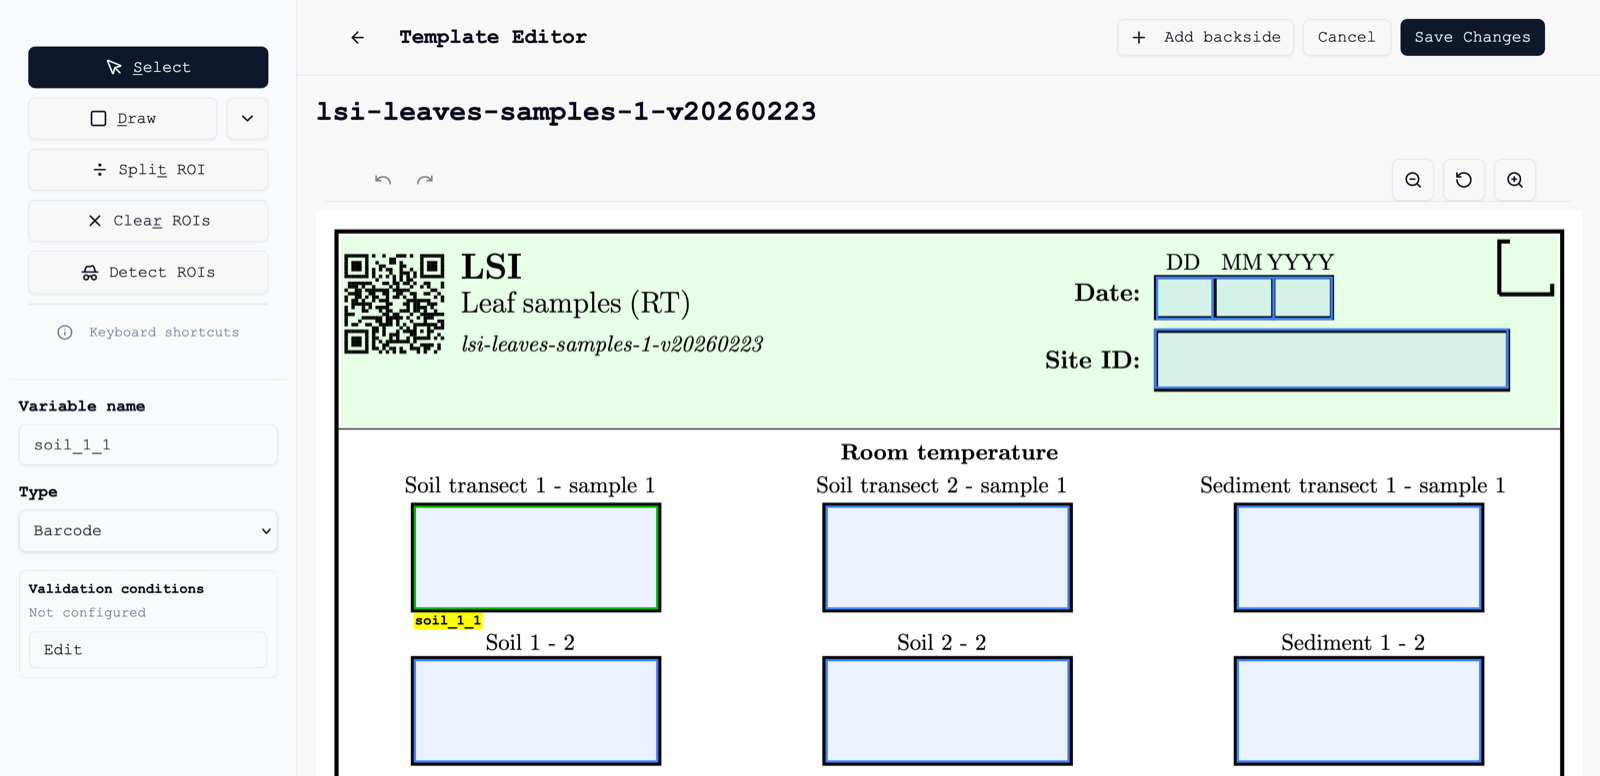
\includegraphics[width=0.95\textwidth]{figures/editor.png}
\caption{Interactive template editor for drawing, naming, and typing ROIs on a PDF template.}
\label{fig:editor}
\end{figure}

\begin{figure}[!ht]
\centering
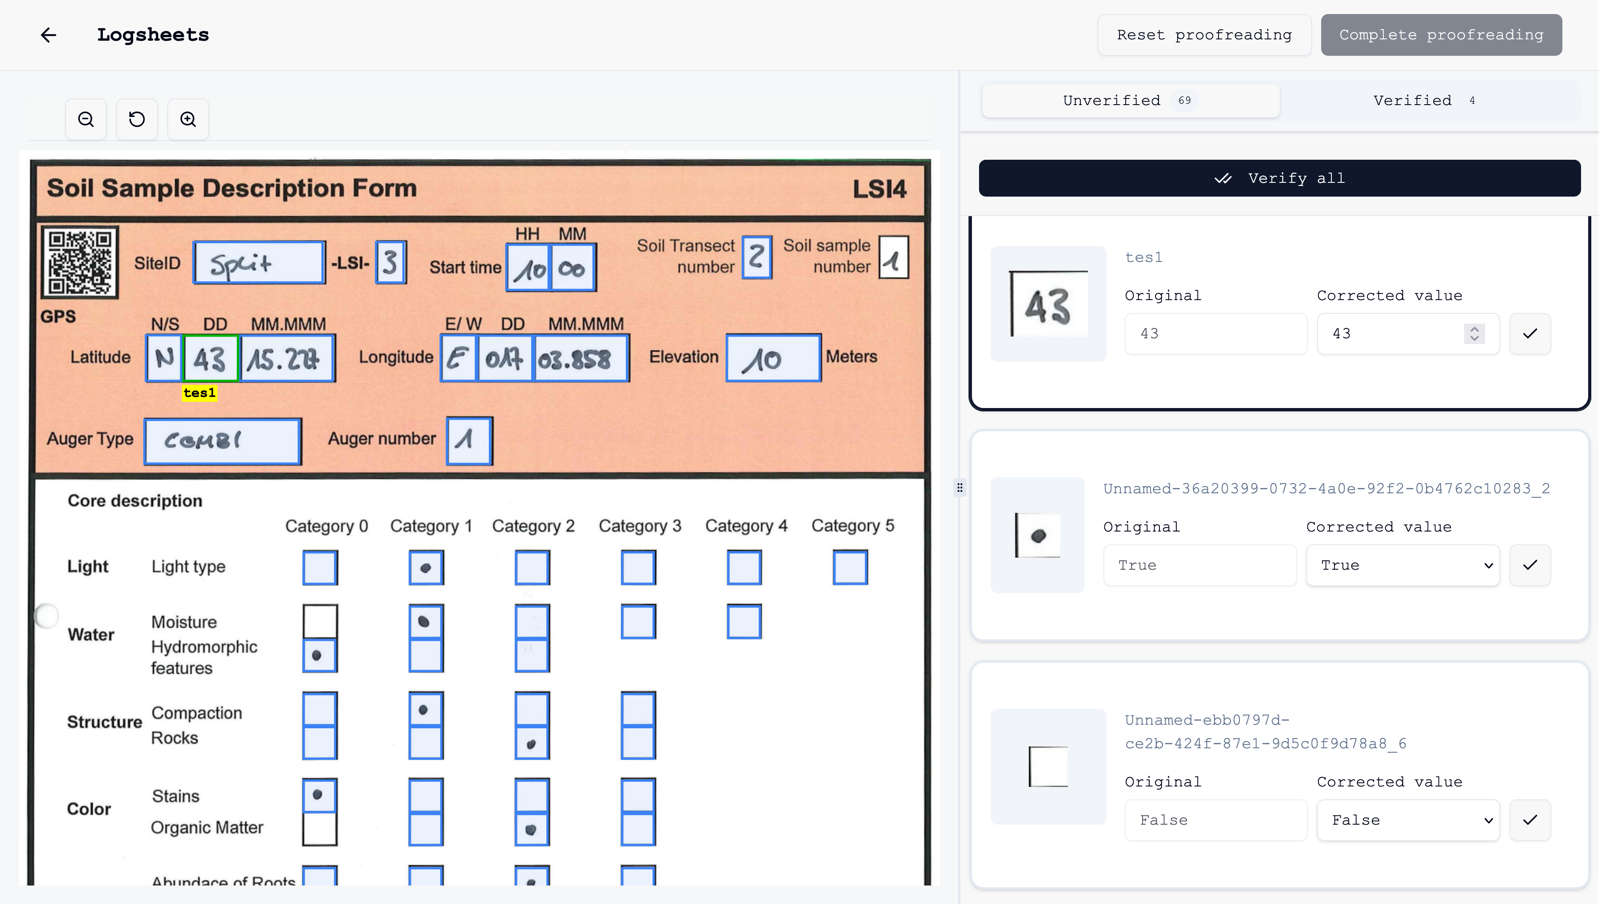
\includegraphics[width=0.95\textwidth]{figures/proofreading.png}
\caption{Side-by-side proofreading workspace linking the scan to extracted field values.}
\label{fig:proofread}
\end{figure}

%% ---------------------------------------------------------------------
\section{Impact}
\label{sec:impact}
%% ---------------------------------------------------------------------

formHTR was developed and continuously optimized during the TRaversing European Coastlines (TREC) expedition~\cite{embl_trec}.
It was used on a collection of approximately ten thousand double-sided logsheets spanning around a hundred different template types, providing contextual metadata for more than eighty thousand collected samples.
Extracted metadata were curated and archived in the BioSamples database~\cite{courtot2022biosamples}, forming an essential foundation for subsequent sample analysis and data production.

LogsheetXtractor extends that same pipeline with a shared web deployment so that the extraction backend serves both the existing CLI and the new interface~\cite{formHTR_pr81}.
Beyond packaging formHTR for non-technical users, the application changes daily practice in two ways that the CLI alone did not support well for its target audience.
First, template definition and revision---drawing, naming, typing, and versioning ROIs---are interactive in the browser; in formHTR these steps relied on desktop GUIs and file-based configs that scientific staff and volunteers found difficult to maintain across many template types.
Second, proofreading is spatially linked to the scan rather than performed in a detached spreadsheet.

\paragraph{Usability evaluation.}
Five first-time users proofread the same logsheet twice---first with formHTR's Excel export alongside the PDF, then with LogsheetXtractor's side-by-side interface (seeded OCR errors in both conditions).
They corrected 76\% of seeded errors on average in the spreadsheet workflow versus 100\% in the application, and mean time per field fell from 10.4\,s to 8.8\,s ($n=5$).
The comparison is small and exploratory; it nevertheless supports the design goal of keeping extracted values visually tied to their ROIs during verification.

%% TODO: new research questions enabled by the software (cite publications if available).
%% TODO: extent of improvement for existing research questions (cite publications if available).
%% TODO: how widespread use is beyond TREC (downloads, active users, other deployments).
%% TODO: commercial / spin-off use, if any (or state N/A).
%% TODO: further evidence of changes to daily practice beyond the n=5 usability study.

%% ---------------------------------------------------------------------
\section{Conclusions}
\label{sec:conclusions}
%% ---------------------------------------------------------------------

%% TODO: write a short conclusions section summarising motivation, design, examples, and impact.
%% Draft placeholder below --- replace with a polished closing paragraph.

LogsheetXtractor provides a deployable web interface over the formHTR extraction pipeline---template-guided multi-provider OCR with spatial binning and consensus voting---enabling scientific staff and volunteers to digitize handwritten field logsheets through interactive template definition, alignment, proofreading, and export without local Python tooling.
Early usability evidence suggests that coupling extracted values to their ROIs during verification improves error correction relative to spreadsheet-only workflows.
%% TODO: add forward-looking sentence (planned features, broader adoption, archival digitization, etc.).

%% ---------------------------------------------------------------------
\section*{Acknowledgements}
\label{sec:acknowledgements}
%% ---------------------------------------------------------------------

This publication was enabled by the support of EMBL member states to the TREC expedition (within the framework of EMBL's Molecules to Ecosystems Programme 2022--2026) and partially funded by the European Union's Horizon 2020 research and innovation programme (project BIOcean5D with grant agreement No.\ 101059915).
Views and opinions expressed are, however, those of the authors only and do not necessarily reflect those of the European Union.
Neither the European Union nor the granting authority can be held responsible for them.
%% TODO: acknowledge additional individuals or institutes as appropriate.

%% ---------------------------------------------------------------------
\section*{AI usage disclosure}
\label{sec:ai-disclosure}
%% ---------------------------------------------------------------------

No generative AI tools were used to implement LogsheetXtractor's application source code, automated tests, or formHTR integration changes.
This manuscript was drafted with assistance from a large language model (Cursor agent) using the author's master's thesis, existing project documentation, and draft formHTR manuscript material as sources; the authors reviewed, edited, and take responsibility for all factual claims, citations, and disclosures in this paper.
%% TODO: confirm wording against SoftwareX / Elsevier generative-AI policies before submission.

%% References via BibTeX
\bibliographystyle{elsarticle-num}
\bibliography{paper}

%% =====================================================================
%% Executable software metadata (mandatory in SoftwareX template)
%% =====================================================================

\section*{Current executable software version}
\label{sec:executable-version}

%% TODO: confirm SoftwareX still requires this second metadata table and the exact row labels
%% from the current Guide for Authors; adjust if the journal template has changed.

\begin{table}[!h]
\begin{tabular}{|l|p{6.5cm}|p{6.5cm}|}
\hline
\textbf{Nr.} & \textbf{Software metadata description} & \textbf{Please fill in this column} \\
\hline
S1 & Current software version & TODO: same as C1 / release tag \\
\hline
S2 & Permanent link to executables of this version & TODO: GitHub Releases / Docker image URL / Zenodo archive \\
\hline
S3 & Legal Software License & MIT \\
\hline
S4 & Computing platforms / Operating Systems & Cross-platform via Docker (Linux containers); developed on macOS/Linux/Windows with Docker Desktop \\
\hline
S5 & Installation requirements \& dependencies & Docker and Docker Compose; cloud OCR provider credentials for recognition; see repository README \\
\hline
S6 & If available, link to user manual --- if formally published & TODO: docs URL or ``see GitHub README'' \\
\hline
S7 & Support email for questions & TODO: same as C8 \\
\hline
\end{tabular}
\caption{Software metadata (mandatory)}
\label{tab:software-metadata}
\end{table}

\end{document}
